\documentclass[11pt,a4paper]{article}

% -----------------------------------------------------------------------------
% Document setup
% -----------------------------------------------------------------------------
\usepackage[T1]{fontenc}
\usepackage[utf8]{inputenc}
\usepackage{lmodern}
\usepackage{microtype}
\usepackage[a4paper,margin=25mm,headheight=14pt]{geometry}

\usepackage{amsmath,amssymb,mathtools}
\usepackage{booktabs}
\usepackage{tabularx}
\usepackage{array}
\usepackage{graphicx}
\usepackage{float}
\usepackage{caption}
\usepackage{subcaption}
\usepackage{xcolor}
\usepackage{enumitem}
\usepackage{listings}
\usepackage{fancyhdr}
\usepackage[hidelinks]{hyperref}

% -----------------------------------------------------------------------------
% Student and assignment details: edit these fields first.
% -----------------------------------------------------------------------------
\newcommand{\studentname}{Rui Luo}
\newcommand{\studentuid}{u8076655}
\newcommand{\coursecode}{COMP8620}
\newcommand{\coursetitle}{Advanced Topics in AI: Intelligent Robotics}
\newcommand{\assignmenttitle}{Assignment 1}
\newcommand{\semester}{Semester 2, 2026}

% -----------------------------------------------------------------------------
% Styling helpers
% -----------------------------------------------------------------------------
\definecolor{anuBlue}{HTML}{1F4E79}
\definecolor{codeBackground}{HTML}{F5F7F9}
\definecolor{codeBorder}{HTML}{D7DCE2}
\definecolor{placeholderGray}{HTML}{606770}

\hypersetup{
  pdftitle={\coursecode\ \assignmenttitle},
  pdfauthor={\studentname\ (\studentuid)},
  colorlinks=true,
  linkcolor=anuBlue,
  citecolor=anuBlue,
  urlcolor=anuBlue
}

\pagestyle{fancy}
\fancyhf{}
\lhead{\coursecode\ -- \assignmenttitle}
\rhead{\studentuid}
\cfoot{\thepage}

\setcounter{secnumdepth}{3}
\setcounter{tocdepth}{2}
\setlist[itemize]{leftmargin=*,itemsep=2pt,topsep=4pt}
\setlist[enumerate]{leftmargin=*,itemsep=2pt,topsep=4pt}
\captionsetup{font=small,labelfont=bf}

\newcommand{\placeholder}[1]{%
  \par\smallskip
  \noindent\textcolor{placeholderGray}{\textit{[Replace this placeholder: #1]}}
  \par\smallskip
}

\newcommand{\finalresult}[1]{%
  \begin{equation}
    \boxed{#1}
  \end{equation}
}

\newcommand{\figureplaceholder}[1]{%
  \begin{center}
    \fcolorbox{codeBorder}{codeBackground}{%
      \parbox[c][45mm][c]{0.86\linewidth}{\centering
        \textcolor{placeholderGray}{\textit{#1}}}}
  \end{center}
}

\lstdefinestyle{python}{
  language=Python,
  basicstyle=\ttfamily\small,
  backgroundcolor=\color{codeBackground},
  frame=single,
  rulecolor=\color{codeBorder},
  numbers=left,
  numberstyle=\scriptsize\color{placeholderGray},
  breaklines=true,
  showstringspaces=false,
  columns=fullflexible,
  keywordstyle=\color{anuBlue}\bfseries,
  commentstyle=\color{placeholderGray}
}

\lstdefinestyle{terminal}{
  basicstyle=\ttfamily\small,
  backgroundcolor=\color{codeBackground},
  frame=single,
  rulecolor=\color{codeBorder},
  breaklines=true,
  showstringspaces=false,
  columns=fullflexible
}

\lstdefinestyle{pseudocode}{
  basicstyle=\ttfamily\small,
  backgroundcolor=\color{codeBackground},
  frame=single,
  rulecolor=\color{codeBorder},
  numbers=left,
  numberstyle=\scriptsize\color{placeholderGray},
  breaklines=true,
  showstringspaces=false,
  columns=fullflexible,
  keywordstyle=\color{anuBlue}\bfseries,
  commentstyle=\color{placeholderGray}\itshape,
  morecomment=[l]{//},
  morekeywords={PROCEDURE,INPUT,OUTPUT,REQUIRE,ENSURE,IF,ELSE,WHILE,FOR,RETURN,FAILURE}
}

\lstdefinestyle{prompt}{
  basicstyle=\ttfamily\small,
  backgroundcolor=\color{codeBackground},
  frame=single,
  rulecolor=\color{codeBorder},
  breaklines=true,
  showstringspaces=false,
  columns=fullflexible
}

\begin{document}
\pagenumbering{gobble}

% -----------------------------------------------------------------------------
% Title page
% -----------------------------------------------------------------------------
\begin{titlepage}
  \centering
  \vspace*{30mm}
  {\Large\coursecode\par}
  \vspace{4mm}
  {\Large\coursetitle\par}
  \vspace{16mm}
  {\huge\bfseries\assignmenttitle\ Report\par}
  \vspace{5mm}
  {\large\semester\par}
  \vfill

  \begin{tabular}{@{}ll@{}}
    \toprule
    Student & \studentname \\
    UID & \studentuid \\
    \bottomrule
  \end{tabular}

  \vfill
  {\large The Australian National University\par}
  \vspace{10mm}
\end{titlepage}

\pagenumbering{arabic}

% -----------------------------------------------------------------------------
% AI disclosure
% -----------------------------------------------------------------------------
\section*{Generative AI Disclosure}
\label{sec:ai-disclosure}

Two generative-AI tools were used. Claude (Anthropic, accessed via Claude
Code) was used throughout: interpreting the assignment, drafting and
revising Parts A and B of this report, implementing \texttt{planner.py} and
\texttt{run\_planner.py}, designing and running the B4/B5 experiments, and
generating the report's figures and appendices. OpenAI Codex was
separately consulted for independent review of the assignment requirements,
Parts A and B, the B3 implementation, the experiments, and report drafts.
All prompts are reproduced verbatim in their original language in
\texttt{AI\_prompts.txt}, included in the submitted source archive.

% =============================================================================
% Part A
% =============================================================================
\section*{Part A}

\subsection*{Question 1(a): Visibility graph (5 points)}

\noindent\textbf{No.}

\noindent
The standard visibility graph requires polygonal forbidden regions and uses
their vertices as graph nodes:
\[
  \mathcal{C}_{\mathrm{obs}}\text{ polygonal}
  \quad\Longrightarrow\quad
  \text{shortest-path bends occur at obstacle vertices}.
\]

\noindent
For the sphere robot,
\[
  k>0
  \quad\Longrightarrow\quad
  \text{non-point robot}
  \quad\Longrightarrow\quad
  \text{construct the problem in configuration space}.
\]
\noindent
Since it only translates on a fixed plane,
\[
  q=(x,y),
  \qquad
  \mathcal{C}\subseteq\mathbb{R}^2.
\]
\noindent
For a polyhedral obstacle $O$,
\[
  \mathcal{C}_{\mathrm{obs}}
  =
  \left\{q\in\mathcal{C}\mid R(q)\cap O\neq\varnothing\right\}.
\]
\noindent
Let $B_k^3$ be the 3D ball of radius $k$ and $\Pi$ the plane on which the
sphere centre moves. Identifying $\Pi$ with $\mathbb{R}^2$,
\[
  \mathcal{C}_{\mathrm{obs}}
  =\left(O\oplus B_k^3\right)\cap\Pi.
\]
\noindent
Moreover,
\[
  \begin{aligned}
    O\text{ polyhedral},\ k>0
    &\quad\Longrightarrow\quad
    O\oplus B_k^3\text{ has rounded edge and vertex regions},\\
    &\quad\Longrightarrow\quad
    \left(O\oplus B_k^3\right)\cap\Pi
    \text{ generally contains curved arcs},\\
    &\quad\Longrightarrow\quad
    \mathcal{C}_{\mathrm{obs}}\text{ is generally non-polygonal}.
  \end{aligned}
\]
\noindent
Therefore,
\[
  \begin{aligned}
    \mathcal{C}_{\mathrm{obs}}\text{ non-polygonal}
    &\quad\Longrightarrow\quad
      \text{the polygonal-forbidden-region assumption is violated},\\
    &\quad\Longrightarrow\quad
      \boxed{\text{the standard visibility graph cannot be applied directly}.}
  \end{aligned}
\]

\clearpage
\subsection*{Question 1(b): Uniform grid discretisation (5 points)}

\noindent\textbf{Yes.}

\noindent
Uniform-grid discretisation requires only a free/occupied test for each cell;
it does not require an explicit polygonal representation of
$\mathcal{C}_{\mathrm{obs}}$.  For the given sphere and obstacles, define
\[
  \operatorname{FREE\text{-}CELL}(c)
  \quad\Longleftrightarrow\quad
  \forall q\in c,\ R_k(q)\cap Obs=\varnothing
  \quad\Longleftrightarrow\quad
  c\cap\mathcal{C}_{\mathrm{obs}}=\varnothing.
\]
Thus, $\operatorname{FREE\text{-}CELL}$ directly collision-checks the
radius-$k$ sphere; it does not require explicitly constructing the curved
boundary of $\mathcal{C}_{\mathrm{obs}}$.

\begin{lstlisting}[
  style=pseudocode,
  caption={Uniform-grid planner for the translating sphere robot},
  label={alg:grid}
]
PROCEDURE UNIFORM-GRID(I, G, h)

INPUT: initial configuration I, goal configuration G,
       and cell width h
OUTPUT: a collision-free path, or FAILURE

// C is the 2-D configuration space of the sphere centre.
// GRID(C, h) is the set of square cells of width h.
// c is one cell; c_i and c_j are edge-sharing cells.
// k is the sphere radius; Obs is the workspace obstacle set.
// FREE-CELL(c) tests the entire cell using the given k and Obs.

    V <- empty set  // free cells used as graph nodes
    E <- empty set  // edges between neighboring free cells

    FOR EACH cell c in GRID(C, h):
        IF FREE-CELL(c):
            V <- V union {c}

    FOR EACH pair c_i, c_j in V that share an edge:
        E <- E union {(c_i, c_j)}

    Gamma <- (V, E)             // the resulting grid graph
    c_I <- CELL-CONTAINING(I)   // cell containing the initial state
    c_G <- CELL-CONTAINING(G)   // cell containing the goal state

    IF c_I is not in V or c_G is not in V:
        RETURN FAILURE

    // P is an ordered sequence of cells from c_I to c_G.
    P <- GRAPH-SEARCH(Gamma, c_I, c_G)

    IF P does not exist:
        RETURN FAILURE

    // CENTRES(P) gives their centres in path order.
    // POLYLINE joins I, these centres, and G by line segments.
    RETURN POLYLINE(I, CENTRES(P), G)
\end{lstlisting}

\noindent
Since every retained cell is obstacle-free, straight-line segments connecting
the centres of adjacent retained cells are collision-free. However, the
planner may miss narrow passages when $h$ is too large, so its success depends
on the grid resolution.

\clearpage
\subsection*{Question 2(a): Upper bound on workspace path length (15 points)}

\noindent
Let
\[
  \Delta\theta_i=\theta_i'-\theta_i,
  \qquad
  \delta=d_C(q,q')
  =\max_{1\leq i\leq K}|\Delta\theta_i|.
\]
Then
\[
  |\Delta\theta_i|\leq\delta,
  \qquad i=1,\ldots,K.
\]
Parameterise the straight configuration-space path by
\[
  q(s)=q+s(q'-q),
  \qquad s\in[0,1],
\]
so that $\dot{\theta}_i(s)=\Delta\theta_i$.

\noindent
Consider an arbitrary material point $P$ on link $m$, where
$1\leq m\leq K$.  Let $r_i(P,s)$ be its distance from joint $i$ at
configuration $q(s)$.  For each upstream joint $i\leq m$,
\[
  r_i(P,s)\leq(m-i+1)L.
\]
Changing $\theta_i$ rotates the subchain from joint $i$ onward about that
joint.  Along the path, an infinitesimal increase $ds$ changes joint $i$ by
\[
  |d\theta_i|=|\Delta\theta_i|\,ds.
\]
If only joint $i$ is considered, $P$ moves along a circular arc centred at
joint $i$ with radius $r_i(P,s)$.  Its infinitesimal path-length contribution
is therefore
\[
  d\ell_i(P,s)=r_i(P,s)|\Delta\theta_i|\,ds.
\]
All upstream joints move simultaneously.  By the triangle inequality, the
actual infinitesimal displacement of $P$ is no greater than the sum of these
contributions.  Hence,
\[
  \begin{aligned}
    \ell(P)
    &\leq \int_0^1
      \sum_{i=1}^{m}r_i(P,s)|\Delta\theta_i|\,ds\\
    &\leq
      L\delta\sum_{i=1}^{m}(m-i+1)\\
    &=\frac{Lm(m+1)}{2}\,\delta\\
    &\leq\frac{LK(K+1)}{2}\,\delta.
  \end{aligned}
\]
Substituting $\delta=d_C(q,q')$ gives, for every point $P$ on the robot,
\[
  \boxed{
    \ell(P)
    \leq
    \frac{LK(K+1)}{2}\,d_C(q,q')
  }.
\]
Thus, a valid upper bound is
\[
  \boxed{\alpha=\frac{LK(K+1)}{2}}.
\]

\clearpage
\subsection*{Question 2(b): Collision-free neighbourhood radius (8 points)}

For any
\[
  q'\in\operatorname{Neigh}(q),
  \qquad
  d_C(q,q')\leq\tau,
\]
parameterise the straight configuration-space path as
\[
  q(s)=q+s(q'-q),
  \qquad s\in[0,1].
\]
Since $s\in[0,1]$, substituting $q(s)$ into the definition of $d_C$ gives
\[
  \begin{aligned}
    d_C(q,q(s))
    &=\max_{1\leq i\leq K}
      \left|\bigl[\theta_i+s({\theta_i}'-\theta_i)\bigr]-\theta_i\right|\\
    &=\max_{1\leq i\leq K}s|{\theta_i}'-\theta_i|\\
    &=s\max_{1\leq i\leq K}|{\theta_i}'-\theta_i|\\
    &=s\,d_C(q,q')\\
    &\leq s\tau\leq\tau,
  \end{aligned}
\]

\noindent
By Part~2(a), every point on the robot travels a workspace path of length at
most $\alpha d_C(q,q(s))\leq\alpha\tau$, so its displacement is at most
$\alpha\tau$.  Moving every robot point by at most $\alpha\tau$ can reduce
the minimum robot--obstacle distance by at most $\alpha\tau$.  Hence, by the
triangle inequality,
\[
  d_W(q(s),Obs)
  \geq d_W(q,Obs)-\alpha\tau.
\]
The right-hand side is the initial clearance minus the maximum possible
approach towards the obstacles.  To guarantee collision-free motion, this
lower bound must be positive:
\[
  d_W(q,Obs)-\alpha\tau>0
  \;\Longrightarrow\;
  \alpha\tau<d_W(q,Obs)
  \;\Longrightarrow\;
  \tau<\frac{d_W(q,Obs)}{\alpha},
\]
where $\alpha>0$.  Under this condition, $d_W(q(s),Obs)>0$ for every
$s\in[0,1]$, so the entire path from $q$ to $q'$ is collision-free.

\noindent
Since $\operatorname{Neigh}(q)$ includes its boundary and obstacle contact
($d_W=0$) is a collision, equality cannot guarantee safety.  Therefore,
\[
  \boxed{
    0\leq\tau<
    \frac{d_W(q,Obs)}{\alpha}
  }
\]
The supremum of the guaranteed radii is
\[
  \boxed{
    \tau_{\mathrm{sup}}
    =
    \frac{d_W(q,Obs)}{\alpha}
    =
    \frac{2\,d_W(q,Obs)}{LK(K+1)}
  },
\]
where $\alpha=LK(K+1)/2$ from Part~2(a).

% =============================================================================
% Part B
% =============================================================================
\clearpage
\section*{Part B}

\subsection*{Question 1: Centralised configuration space (2 points)}

For $K\in\{1,\ldots,5\}$, let $\mathcal W$ be the bounded physical
workspace and
\[
  \mathcal W_r=\{p\in\mathcal W\mid B_r(p)\subseteq\mathcal W\}
\]
be the admissible region for a drone centre.  If
\[
  p_i=(x_i,y_i,z_i)\in\mathbb R^3
\]
is the centre of drone $i$, centralised planning treats the $K$ drones as one
composite robot, so a joint configuration is
\[
  q=(p_1,\ldots,p_K)
  \in\mathcal C=\mathcal W_r^K\subseteq\mathbb R^{3K},
  \qquad
  \boxed{\dim(\mathcal C)=3K}.
\]
Let $B_r(p_i)$ be drone $i$'s bounding sphere and let $Obs$ be the union of
the workspace obstacles.  The collision-free subset is
\[
  \mathcal C_{\mathrm{free}}
  =
  \left\{
    q\in\mathcal C
    \;\middle|\;
    \begin{array}{ll}
      B_r(p_i)\cap Obs=\varnothing,
        & i=1,\ldots,K,\\
      \|p_i-p_j\|_2>2r,
        & 1\leq i<j\leq K
    \end{array}
  \right\}.
\]

\subsection*{Question 2: Sampling-based planner design (6 points)}

I use bidirectional RRT-Connect~\cite{rrtconnect} for three reasons:
\begin{enumerate}[label=(\arabic*),nosep]
  \item This is a single-query problem in a continuous $3K$-dimensional
        configuration space, with validity checks available from the simulator.
  \item Growing trees from both endpoints and greedily connecting them focuses
        computation on finding a feasible path within the 20-second limit.
  \item PRM's reusable roadmap is unnecessary for one query, while RRT* spends
        additional computation on path optimisation that is not required here.
\end{enumerate}
For $q=(p_1,\ldots,p_K)$ and $q'=(p'_1,\ldots,p'_K)$, use
\[
  d(q,q')=\max_{1\leq i\leq K}\|p_i-p'_i\|_2,
  \qquad
  \operatorname{Steer}(q,q')=q+
  \min\left\{1,\frac{\eta}{d(q,q')}\right\}(q'-q),
\]
where $\eta>0$ is the extension length, set to $5\%$ of the workspace
diagonal so it scales with the problem instance rather than being a fixed
constant.  \textsc{Sample-Free} samples uniformly within the bounds and
rejects states failing \texttt{sim.is\_valid};
\textsc{Nearest} minimises $d$ by brute-force linear scan over the tree,
which is appropriate here because a single \texttt{motion\_valid} call
(interpolated at fixed step size) costs far more than comparing $d$ against
the handful-to-low-hundreds of nodes a 20-second budget produces at
$K\leq5$, so a spatial index would not pay for itself.  An edge is accepted
only by \texttt{sim.motion\_valid}.  The goal-tree root $q_G$ satisfies both
\texttt{sim.is\_valid} and \texttt{sim.is\_goal}.

\begin{lstlisting}[
  style=pseudocode,
  caption={Centralised RRT-Connect},
  label={alg:planner}
]
PROCEDURE RRT-CONNECT(sim, eta, T_max)

INPUT: simulator sim, extension length eta, and time limit T_max
OUTPUT: a collision-free joint path, or FAILURE

// q_I is the initial configuration; q_G is a valid configuration
// satisfying the goal condition.
// Each tree node stores a joint configuration and a parent pointer.
// T_I and T_G are rooted at q_I and q_G, respectively.
// T_a is the active tree; T_b is the opposite tree.
// eta is the maximum length of one extension.

    deadline <- CLOCK() + T_max
    q_I <- sim.initial_configuration
    q_G <- VALID-GOAL-SAMPLE(sim, deadline)

    IF q_G does not exist or NOT sim.is_valid(q_I):
        RETURN FAILURE

    IF sim.motion_valid(q_I, q_G):
        RETURN [q_I, q_G]

    T_I, T_G <- trees rooted at q_I and q_G
    T_a, T_b <- T_I, T_G

    WHILE CLOCK() < deadline:
        // q_rand is a randomly sampled collision-free configuration.
        q_rand <- SAMPLE-FREE(sim, deadline)

        IF q_rand does not exist:
            RETURN FAILURE

        // q_new is the node returned by extending the active tree.
        status, q_new <- EXTEND(T_a, q_rand, eta, sim)

        IF status != TRAPPED:
            // q_meet is the node reached by the opposite tree.
            status_b, q_meet <- CONNECT(T_b, q_new, eta, sim, deadline)

            IF status_b == REACHED:
                // T_a identifies which parent chain contains q_new.
                RETURN JOIN-PATHS(T_I, T_G, q_new, q_meet, T_a)

        T_a, T_b <- T_b, T_a

    RETURN FAILURE

// EXTEND takes one collision-free step from T toward q_target.
PROCEDURE EXTEND(T, q_target, eta, sim)
    q_near <- NEAREST(T, q_target, d)

    IF d(q_near, q_target) == 0:
        RETURN REACHED, q_near

    q_new <- STEER(q_near, q_target, eta)

    IF NOT sim.motion_valid(q_near, q_new):
        RETURN TRAPPED, q_near

    add q_new to T with parent q_near

    IF q_new == q_target:
        RETURN REACHED, q_new

    RETURN ADVANCED, q_new

// CONNECT repeatedly extends T until it is trapped or reaches q_target.
PROCEDURE CONNECT(T, q_target, eta, sim, deadline)
    q_last <- NEAREST(T, q_target, d)

    WHILE CLOCK() < deadline:
        status, q_last <- EXTEND(T, q_target, eta, sim)

        IF status != ADVANCED:
            RETURN status, q_last

    RETURN TIMEOUT, q_last

// JOIN-PATHS splices the branch ending at q_new (grown in T_a) with the
// branch ending at q_meet (grown in T_b) into one q_I -> q_G path.
PROCEDURE JOIN-PATHS(T_I, T_G, q_new, q_meet, T_a)
    branch_new  <- trace q_new back to its tree's root, root-to-node order
    branch_meet <- trace q_meet back to its tree's root, root-to-node order

    IF T_a == T_I:
        RETURN branch_new followed by reverse(branch_meet)
    ELSE:
        RETURN branch_meet followed by reverse(branch_new)

// Return a collision-free joint configuration inside the goal regions.
PROCEDURE VALID-GOAL-SAMPLE(sim, deadline)
    q_G <- the vector of goal centres

    IF sim.is_valid(q_G) AND sim.is_goal(q_G):
        RETURN q_G

    WHILE CLOCK() < deadline:
        q_G <- sample one point inside each drone's goal region

        IF sim.is_valid(q_G) AND sim.is_goal(q_G):
            RETURN q_G

    RETURN FAILURE
\end{lstlisting}

\noindent
All tree edges pass \texttt{motion\_valid}.  \textsc{Join-Paths} uses $T_a$ to
orient their parent chains into a collision-free path from $q_I$ to the valid
goal $q_G$; a finite deadline may return \textsc{Failure}.

\subsection*{Question 3: Implementation and demonstration (15 points)}

The submitted \texttt{planner.py} implements Algorithm~\ref{alg:planner} with
the supplied MultiDrone collision and local-motion primitives~\cite{multidrone}.
\texttt{run\_planner.py} loads a simulator-format YAML file, infers $K$, sets
the seed and scaled $\eta$, and enforces the 20-second total demo budget.

\paragraph{Reproduction commands.}
\begin{lstlisting}[style=terminal]
# Complete template; arguments in brackets are optional.
python3 run_planner.py --environment <scenario.yaml> \
  [--num-drones K] [--time-limit SECONDS] [--seed SEED] [--eta ETA] \
  [--bridge-prob P] [--bridge-sigma SIGMA] [--local-bridge] [--visualize]
#   --num-drones   inferred from the YAML if omitted
#   --time-limit   demo budget in seconds (default 20)
#   --seed         RNG seed (default 0)
#   --eta          max extension length (default 5% of the workspace diagonal)
#   --bridge-prob  bridge-test sampling probability (default 0 = B2 baseline)
#   --bridge-sigma bridge-test perturbation stdev (default eta)
#   --local-bridge anchor bridge attempts near the active tree (EST-style)
#   --visualize    open the simulator's 3D viewer after a success

# Minimal template.
python3 run_planner.py --environment <scenario.yaml> --visualize

# Example.
python3 run_planner.py --environment environments/E1_sparse.yaml --visualize
\end{lstlisting}
By default, the runner infers $K$, uses a 20-second limit, seed 0, scaled
$\eta$, and baseline uniform sampling.

\paragraph{Path validation.}
Before reporting success, the runner independently rechecks the initial
configuration, every consecutive edge with \texttt{sim.motion\_valid}, and the
final configuration with \texttt{sim.is\_goal}.

E12 checks goal-region sampling when the goal centres themselves are invalid;
all $25/25$ runs succeeded in $0.06\pm0.01$\,s. E13 seals the initial cluster
inside a closed box; all $10/10$ runs returned \textsc{Failure} without a hang
or invalid path, with capped planner runtime $20.01\pm0.00$\,s excluding
simulator setup.

\subsection*{Question 4: Environment-complexity experiment (6 points)}

\subsubsection*{Research question and hypothesis}
The experiment asks how obstacle density and free-space structure affect
baseline RRT-Connect for five drones. Four hypotheses are tested:
\begin{enumerate}[label=(\arabic*),nosep]
  \item Increasing obstacle density increases planning time.
  \item Narrow or sequential passages reduce success, because fewer random
        samples can connect the two regions.
  \item Multiple alternative passages of the same width improve success
        relative to a single passage.
  \item Compound constraints and local traps reduce finite-time success.
\end{enumerate}

\subsubsection*{Experimental design}
Layouts for every environment referenced below are collected in
Appendix~\ref{app:layouts}.
\begin{table}[H]
  \centering
  \caption{Controlled environment-complexity comparisons.}
  \label{tab:experiment-design}
  \begin{tabularx}{\textwidth}{@{}p{0.22\textwidth}p{0.18\textwidth}Xr@{}}
    \toprule
    Comparison & Environments & Varied feature & Trials each \\
    \midrule
    Obstacle density & E0--E3 & $0,3,7,14$ obstacles; no critical bottleneck & 25 \\
    Passage width & E4, E5 & One gap of width $14$ or $2$ & 25 \\
    Route redundancy & E5, E6 & One or three width-$2$ gaps & 25 \\
    Offset passages & E7 & Two sequential width-$2$ gaps & 15 \\
    Stress tests & E9--E11 & 2-D aperture, coupled swap, or dead-end trap & 25 \\
    \bottomrule
  \end{tabularx}
\end{table}

\paragraph{Protocol.}
\begin{itemize}[nosep]
  \item \textbf{Drones and goals:} $K=5$, the same start and goal
        configurations used across every environment.
  \item \textbf{Workspace:} $[0,50]^3$, drone radius $0.3$.
  \item \textbf{Planner parameters:} $\eta=0.05\sqrt{3(50)^2}=4.330$
        (5\% of the workspace diagonal), uniform sampling only (no bridge
        sampling), 20-second timeout per run.
  \item \textbf{Seeds:} $0$--$24$ for E0--E6 and E9--E11;
        $0$--$14$ for E7.
  \item \textbf{Execution:} runs were sequential; timing used
        \texttt{time.perf\_counter} around the planner call only, excluding
        simulator construction.
  \item \textbf{Hardware/software:} 2.4\,GHz eight-core Intel Core i9
        MacBook Pro, 16\,GB RAM, macOS 26.5.2, NumPy, the supplied
        MultiDrone simulator.
\end{itemize}

\paragraph{Metrics and confidence intervals.}
Success means returning a validated path within 20 seconds. Capped runtime is
the elapsed planner time, with failed runs retaining their observed timeout
duration (approximately 20 seconds). For $n$ runs with sample standard
deviation $s$, the two-sided Student-$t$ interval is
\[
  \bar t \;\pm\; t_{0.975,n-1}\frac{s}{\sqrt n}.
\]
Explicit waypoint witnesses for E9 and E11 were separately validated
state-by-state and edge-by-edge with \texttt{is\_valid} and
\texttt{motion\_valid}. Thus, their zero baseline successes indicate
finite-time planner difficulty rather than infeasibility.

\subsubsection*{Results}
\begin{table}[H]
  \centering
  \caption{Baseline RRT-Connect performance; capped runtime is mean
  $\pm$ 95\% Student-$t$ CI.}
  \label{tab:experiment-results}
  \begin{tabular}{@{}llrrr@{}}
    \toprule
    Environment & Structure & $n$ & Success & Capped runtime (s) \\
    \midrule
    E0 & Empty & 25 & 25/25 & $0.04 \pm 0.00$ \\
    E1 & Sparse & 25 & 25/25 & $0.12 \pm 0.01$ \\
    E2 & Moderate & 25 & 25/25 & $0.32 \pm 0.07$ \\
    E3 & Dense & 25 & 25/25 & $1.03 \pm 0.19$ \\
    E4 & Wide passage & 25 & 25/25 & $0.16 \pm 0.03$ \\
    E5 & Narrow passage & 25 & 20/25 & $10.19 \pm 2.67$ \\
    E6 & Three narrow passages & 25 & 25/25 & $2.95 \pm 0.50$ \\
    E7 & Offset sequential passages & 15 & 1/15 & $19.38 \pm 1.35$ \\
    \midrule
    E9 & Coupled $y$-$z$ aperture & 25 & 0/25 & $20.00 \pm 0.00$ \\
    E10 & Bottleneck + drone swap & 25 & 22/25 & $7.97 \pm 2.38$ \\
    E11 & Dead-end trap & 25 & 0/25 & $20.00 \pm 0.00$ \\
    \bottomrule
  \end{tabular}
\end{table}

\begin{figure}[H]
  \centering
  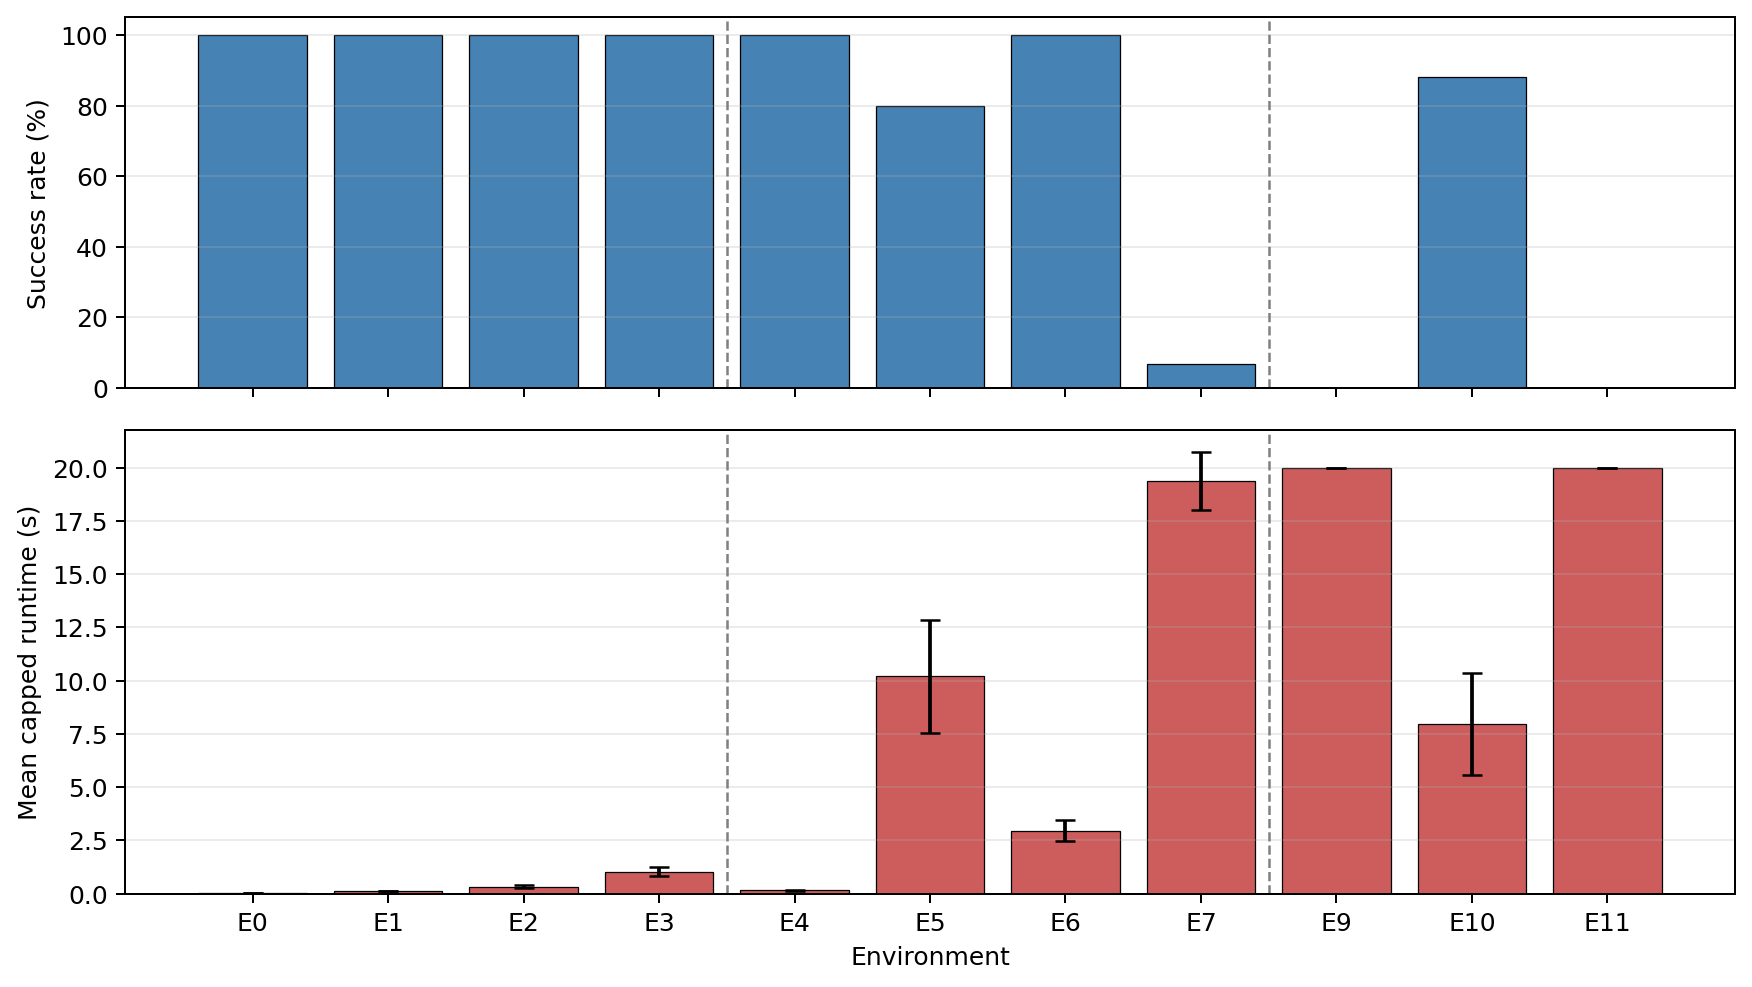
\includegraphics[width=0.86\textwidth]{../A1_code/results/figures/complexity_results.png}
  \caption{Success rate and mean capped runtime for the baseline planner.
  Dashed lines separate density (E0--E3), passage-structure (E4--E7), and
  additional stress tests (E9--E11). Failed runs retain their timeout
  duration; error bars show 95\% Student-$t$ confidence intervals.}
  \label{fig:complexity-results}
\end{figure}

\subsubsection*{Discussion}
\begin{enumerate}[label=(\arabic*),nosep]
  \item \textbf{Obstacle density (E0--E3).} $100\%$ success throughout;
        mean runtime rose from $0.04$ to $1.03$\,s. Consistent with more
        collision rejection and local-motion work, while broad alternative
        routes preserved free-space coverage.
  \item \textbf{Passage geometry vs.\ obstacle count (E4--E7).} Geometry
        matters more than raw count: narrowing E4's single gap from $14$ to
        $2$ units (E5) dropped success from $100\%$ to $80\%$ and raised
        runtime from $0.16$ to $10.19$\,s; three width-$2$ alternatives
        (E6) restored $100\%$ success; two offset transitions (E7)
        succeeded only once in 15 runs. Paths for E5--E7 are in
        Appendix~\ref{app:paths}.
  \item \textbf{Additional axes (E9--E11).} E9's two-dimensional aperture
        and E11's dead-end trap both produced $0/25$ baseline successes,
        although the verified witnesses establish that both are feasible.
        E10 combines E5's bottleneck with a full drone-order reversal; its
        $22/25$ success rate indicates that the bottleneck remained the
        dominant difficulty. Layouts are in Appendix~\ref{app:layouts}.
  \item \textbf{Limitations.} Results use one start--goal set, $K=5$, the
        selected parameters, and a 20-second cutoff; E0--E3 vary obstacle
        geometry rather than forming perfectly nested scenes, and E7 has
        fewer trials. The results are comparative, not universal.
\end{enumerate}

\subsection*{Question 5: Scalability with the number of drones (4 points)}

Increasing $K$ affects the planner in four distinct ways:
\begin{enumerate}[label=(\arabic*),nosep]
  \item \textbf{Dimension.} For $K$ translating drones, $q\in\mathbb{R}^{3K}$,
        so the configuration-space dimension grows linearly as $3K$.
  \item \textbf{Collision-check cost.} A single state check requires $K$
        drone--obstacle checks and $\binom{K}{2}=O(K^2)$ inter-drone checks;
        \textsc{Motion-Valid} repeats these along each local path.
  \item \textbf{Nearest-neighbour cost.} With a brute-force tree of $N$
        nodes, both the nearest-neighbour query and node storage cost
        $O(NK)$.
  \item \textbf{Sample efficiency.} Increasing $K$ reduces the fraction of
        jointly valid samples and the relative measure of coordinated
        passages in the joint space.
\end{enumerate}

To isolate the effect of $K$, E8 contains no static obstacles but reverses the
drones' initial order, making the direct joint-space segment invalid. Each
condition used the baseline planner and 25 seeds. Layouts and successful
paths for $K=2,3,4,5$ are in Appendices~\ref{app:layouts}
and~\ref{app:paths}.

\begin{table}[H]
  \centering
  \caption{Scalability in E8; runtime is mean $\pm$ 95\% Student-$t$ CI
  over 25 runs.}
  \label{tab:scalability-results}
  \begin{tabular}{@{}rrrrr@{}}
    \toprule
    $K$ & Dimension & Pair constraints & Success & Runtime (ms) \\
    \midrule
    2 & 6  & 1  & 25/25 & $21.72 \pm 0.61$ \\
    3 & 9  & 3  & 25/25 & $34.84 \pm 1.40$ \\
    4 & 12 & 6  & 25/25 & $44.68 \pm 4.27$ \\
    5 & 15 & 10 & 25/25 & $54.32 \pm 3.79$ \\
    \bottomrule
  \end{tabular}
\end{table}

\begin{enumerate}[label=(\arabic*),nosep]
  \item \textbf{Result.} All tested E8 runs ($K=2,\ldots,5$) succeeded;
        mean runtime
        increased by a factor of $2.5$ from $K=2$ to $K=5$, consistent
        with the growing state dimension and pairwise checks.
  \item \textbf{Scope.} E8 is obstacle-free, so it does not measure the
        stronger dimensional effect of cluttered narrow passages, already
        visible at $K=5$ in E5 and E7.
  \item \textbf{Conclusion.} The $K=1$ case has dimension $3$ and no
        inter-drone pair constraints; E8 starts at $K=2$ because a swap
        requires two drones. Across the required $K\in[1,5]$ range, the
        implementation is practical in open scenes; in clutter, the
        dominant limitation is repeated local collision checking together
        with the low probability of sampling useful coordinated
        configurations.
\end{enumerate}

% -----------------------------------------------------------------------------
% References
% -----------------------------------------------------------------------------
\clearpage
\begin{thebibliography}{9}

\bibitem{course-notes}
H. Kurniawati,
\emph{COMP8620 Advanced Topics in AI: Intelligent Robotics, Weeks 1--3 lecture materials},
Australian National University, 2026.

\bibitem{multidrone}
RDLLab,
``MultiDrone Simulator,'' 2026.
Available: \url{https://github.com/RDLLab/MultiDrone}.
Accessed: 26 August 2026.

\bibitem{rrtconnect}
J.~J. Kuffner, Jr. and S.~M. LaValle,
``RRT-Connect: An efficient approach to single-query path planning,''
in \emph{Proceedings of the 2000 IEEE International Conference on Robotics
and Automation}, vol.~2, 2000, pp.~995--1001.

\end{thebibliography}

% -----------------------------------------------------------------------------
% Appendices
% -----------------------------------------------------------------------------
\appendix
\clearpage
\section{Environment Layouts}
\label{app:layouts}

Dots denote initial drone positions; translucent circles denote the
corresponding goal regions.

\begin{figure}[H]
  \centering
  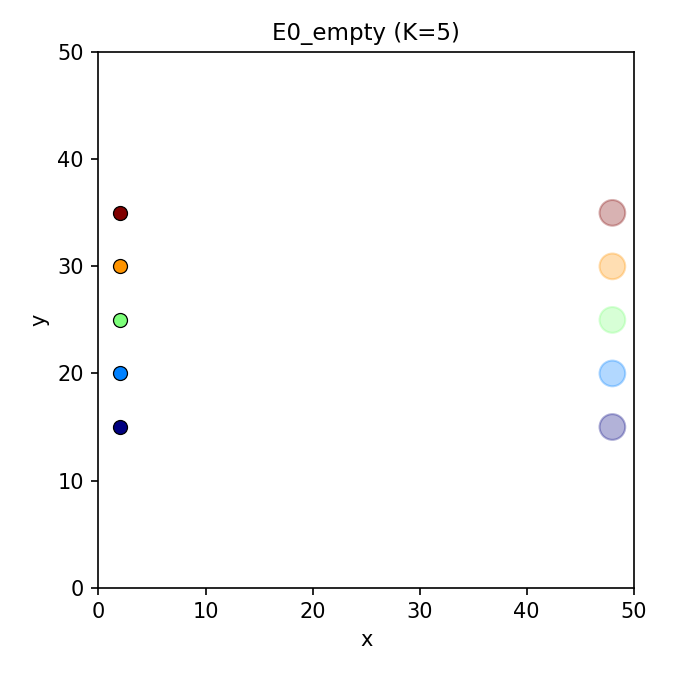
\includegraphics[width=0.24\textwidth]{../A1_code/results/figures/E0_empty.png}
  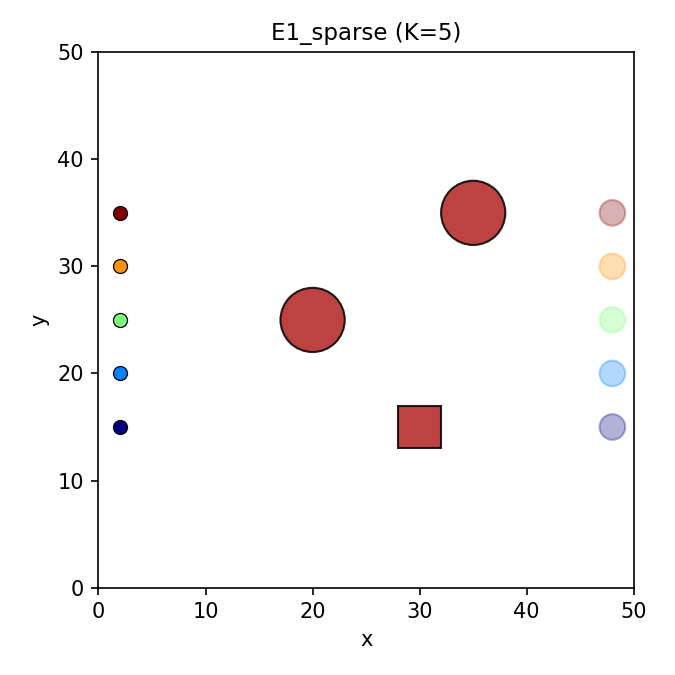
\includegraphics[width=0.24\textwidth]{../A1_code/results/figures/E1_sparse.png}
  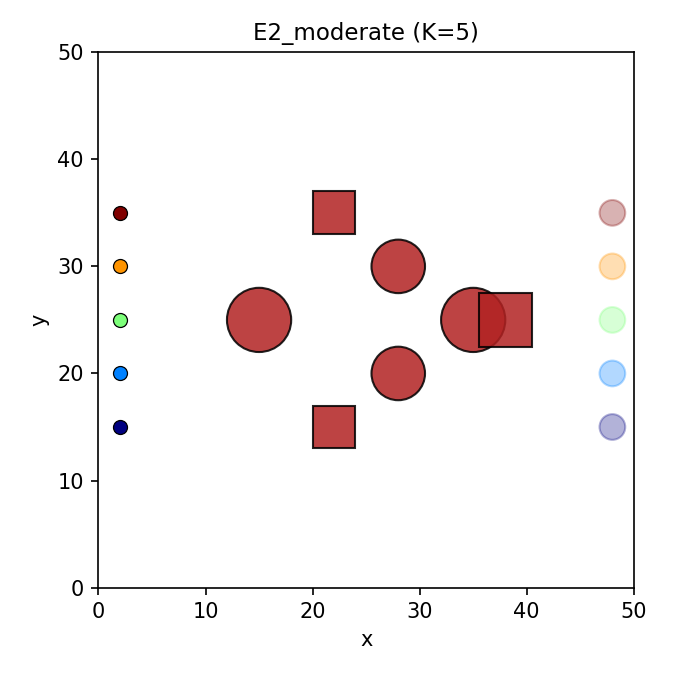
\includegraphics[width=0.24\textwidth]{../A1_code/results/figures/E2_moderate.png}
  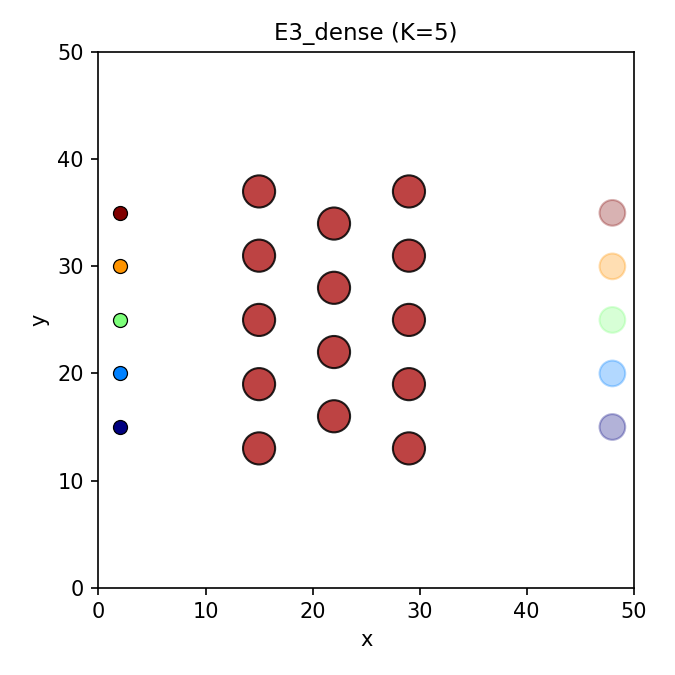
\includegraphics[width=0.24\textwidth]{../A1_code/results/figures/E3_dense.png}
  \caption{E0--E3: obstacle-density comparison (0, 3, 7, 14 obstacles).}
\end{figure}

\begin{figure}[H]
  \centering
  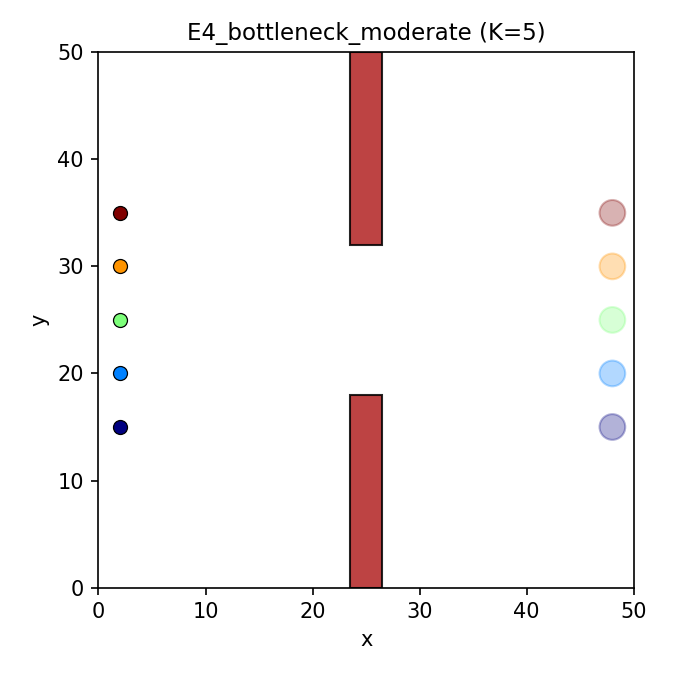
\includegraphics[width=0.24\textwidth]{../A1_code/results/figures/E4_bottleneck_moderate.png}
  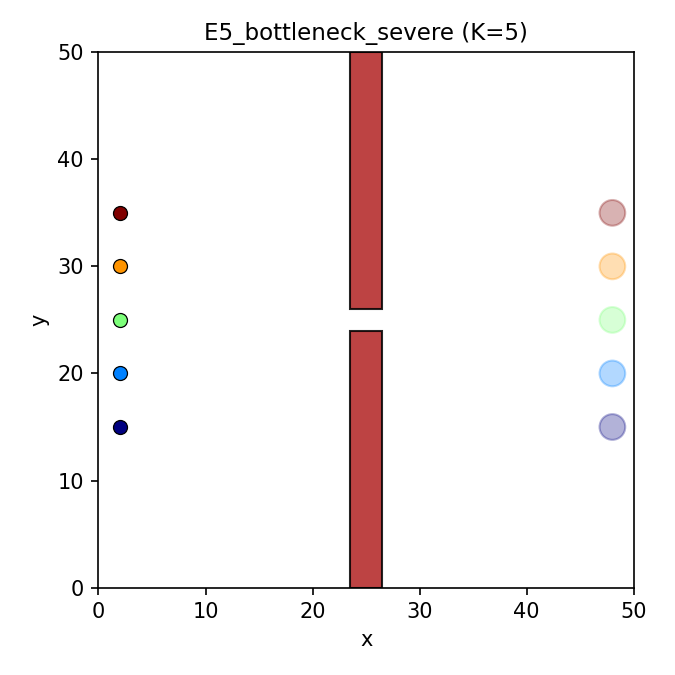
\includegraphics[width=0.24\textwidth]{../A1_code/results/figures/E5_bottleneck_severe.png}
  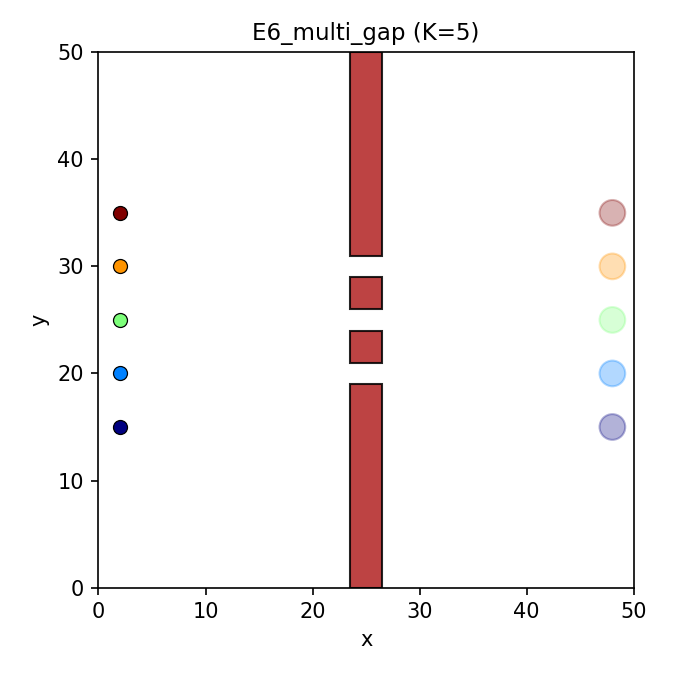
\includegraphics[width=0.24\textwidth]{../A1_code/results/figures/E6_multi_gap.png}
  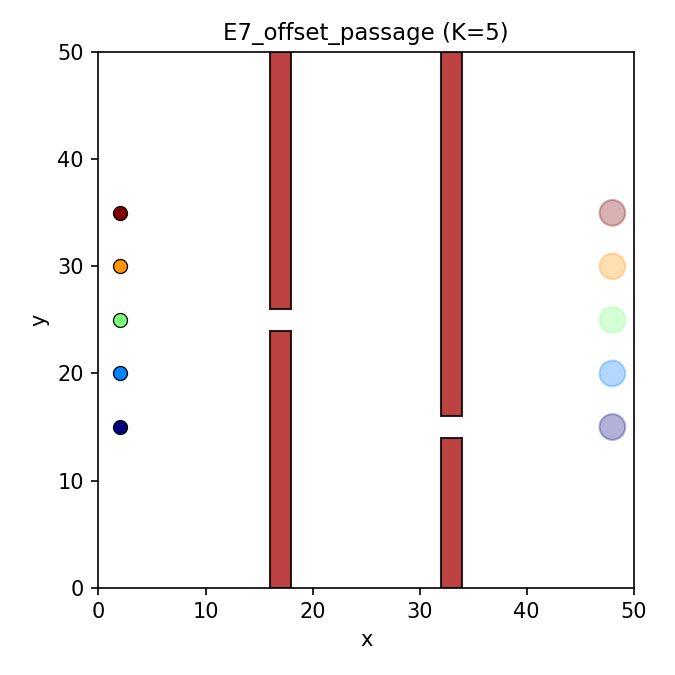
\includegraphics[width=0.24\textwidth]{../A1_code/results/figures/E7_offset_passage.png}
  \caption{E4--E7: passage width, route redundancy, and offset passages.}
\end{figure}

\begin{figure}[H]
  \centering
  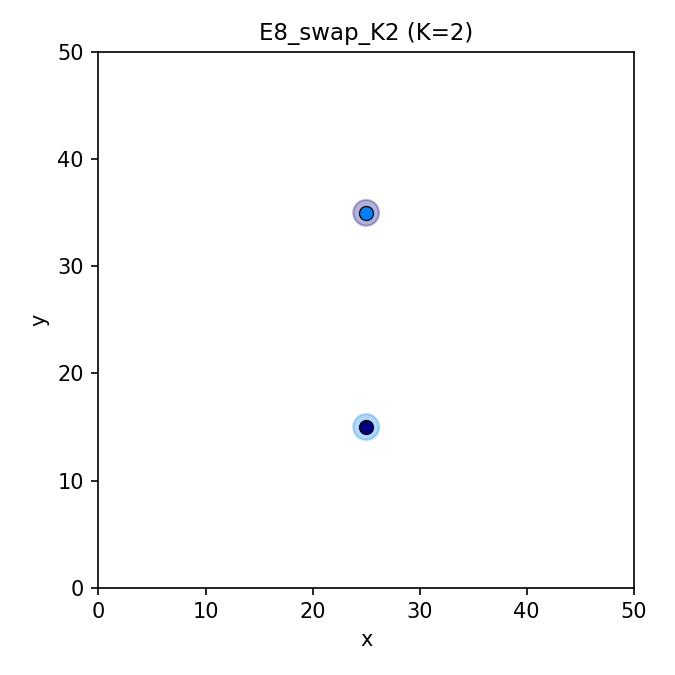
\includegraphics[width=0.24\textwidth]{../A1_code/results/figures/E8_swap_K2.png}
  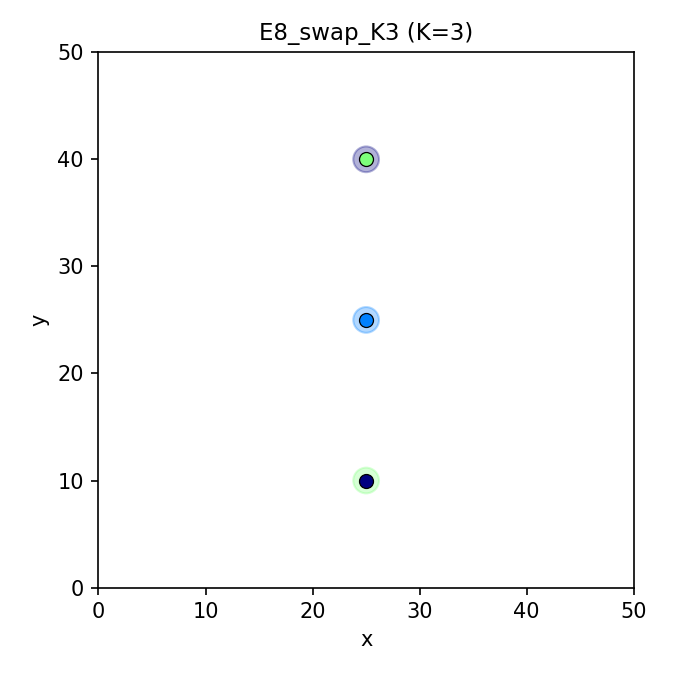
\includegraphics[width=0.24\textwidth]{../A1_code/results/figures/E8_swap_K3.png}
  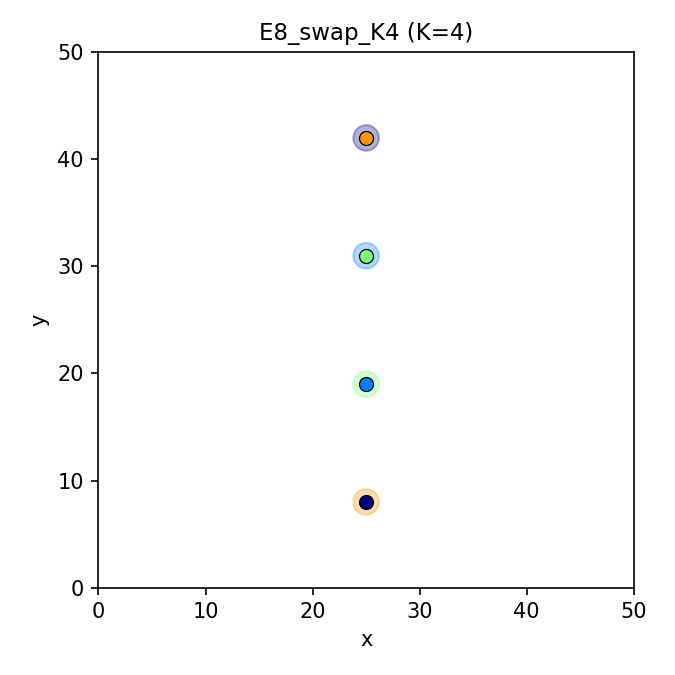
\includegraphics[width=0.24\textwidth]{../A1_code/results/figures/E8_swap_K4.png}
  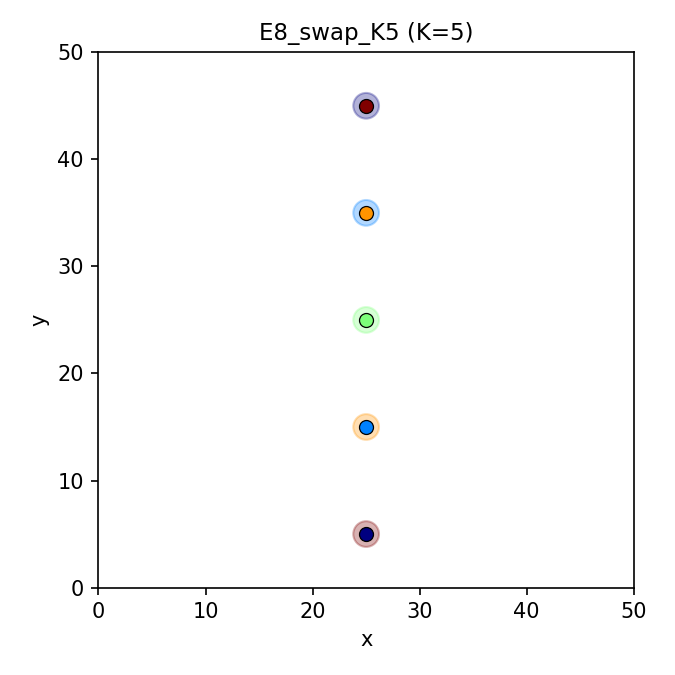
\includegraphics[width=0.24\textwidth]{../A1_code/results/figures/E8_swap_K5.png}
  \caption{E8: drone-swap scalability series, $K=2,3,4,5$ (Question 5).}
\end{figure}

\begin{figure}[H]
  \centering
  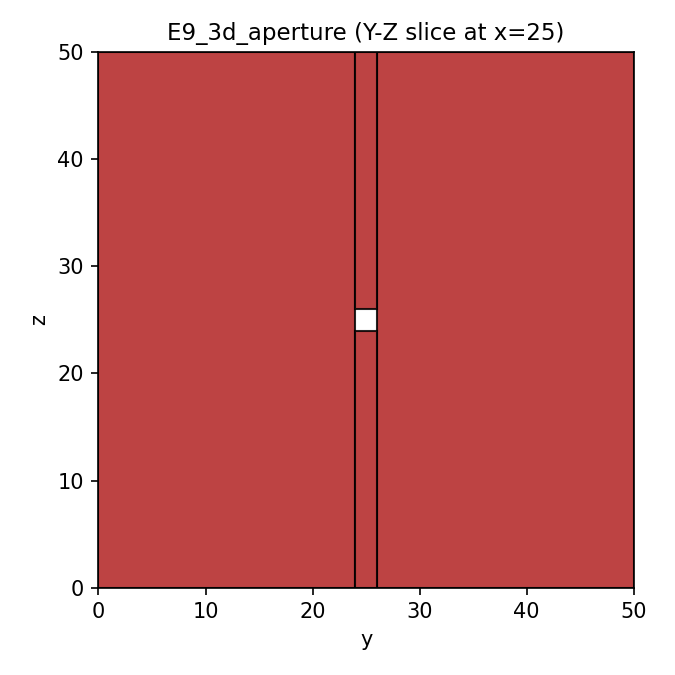
\includegraphics[width=0.19\textwidth]{../A1_code/results/figures/E9_3d_aperture.png}
  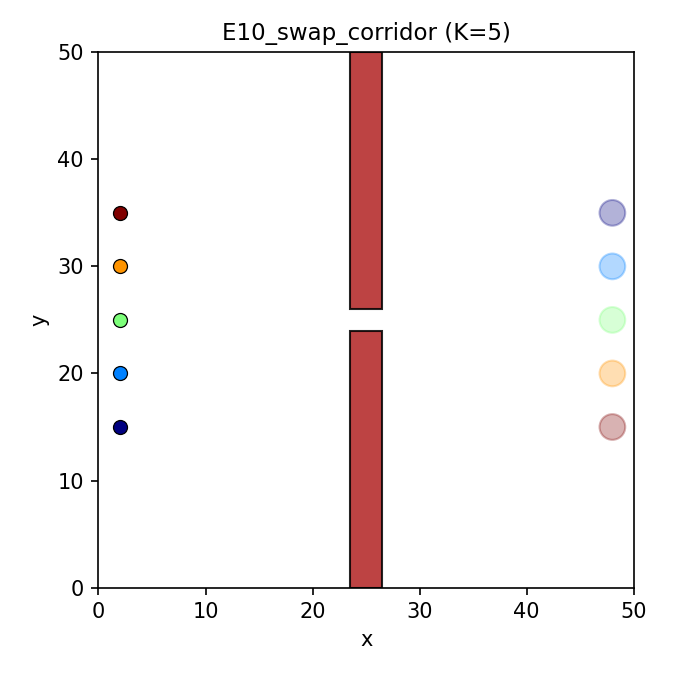
\includegraphics[width=0.19\textwidth]{../A1_code/results/figures/E10_swap_corridor.png}
  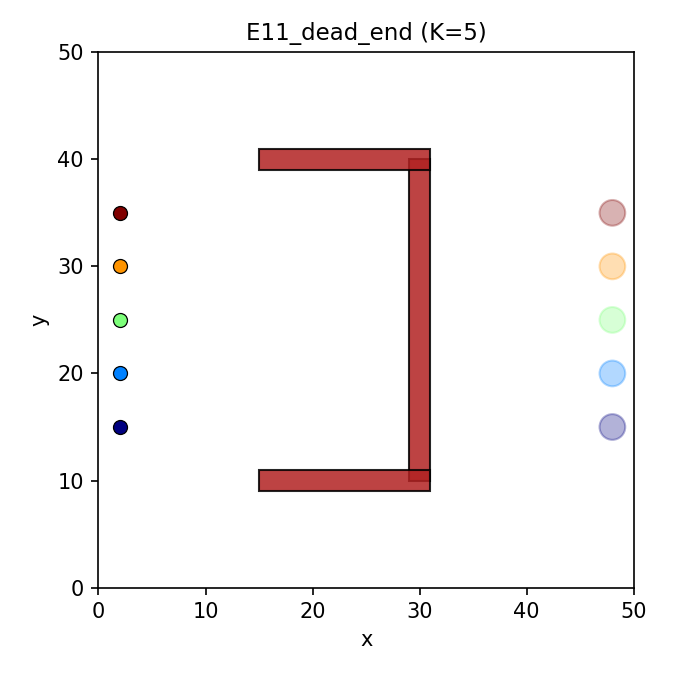
\includegraphics[width=0.19\textwidth]{../A1_code/results/figures/E11_dead_end.png}
  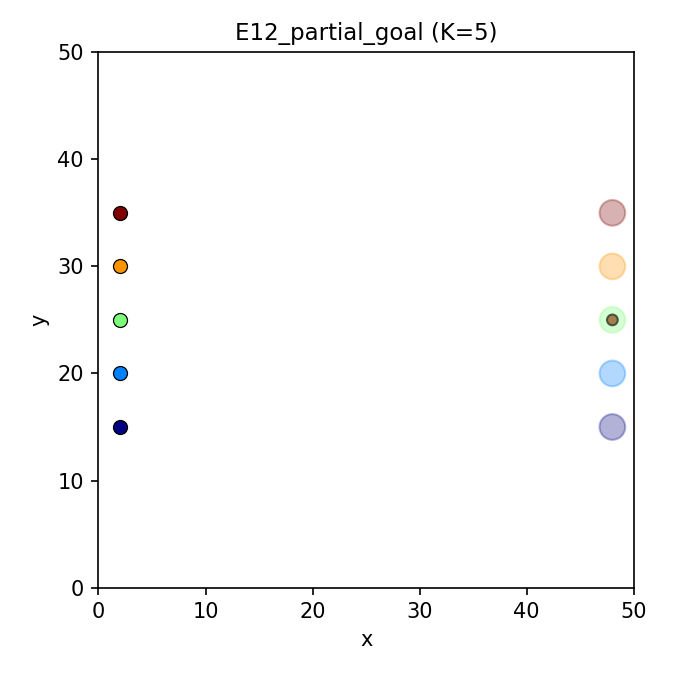
\includegraphics[width=0.19\textwidth]{../A1_code/results/figures/E12_partial_goal.png}
  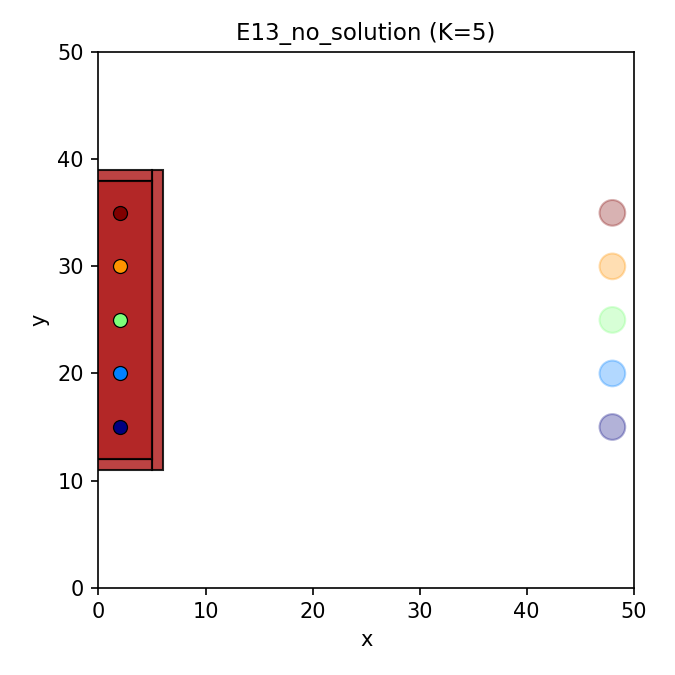
\includegraphics[width=0.19\textwidth]{../A1_code/results/figures/E13_no_solution.png}
  \caption{E9--E13: additional environments (E9--E11 in
  Table~\ref{tab:experiment-results}; E12--E13 are the Question 3 path-validation
  checks). E9 is shown as its $y$-$z$ cross-section, the rest top-down.}
\end{figure}

\clearpage
\section{Successful Paths}
\label{app:paths}

One successful path per environment. E9, E11, E13 omitted ($0\%$ success,
Table~\ref{tab:experiment-results}).

\begin{figure}[H]
  \centering
  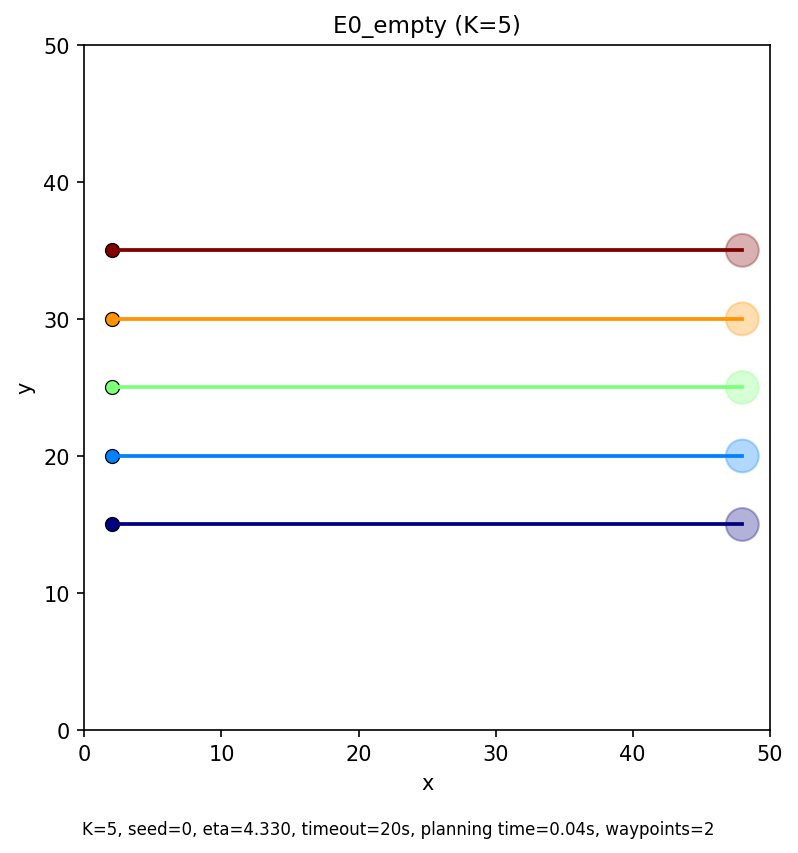
\includegraphics[width=0.24\textwidth]{../A1_code/results/figures/path_E0_empty.png}
  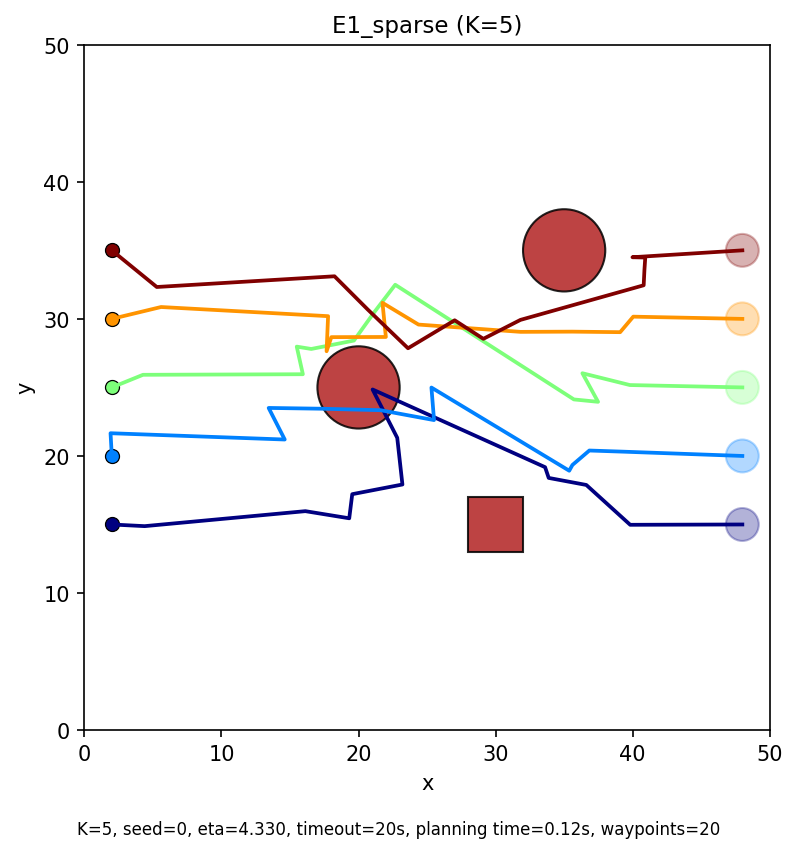
\includegraphics[width=0.24\textwidth]{../A1_code/results/figures/path_E1_sparse.png}
  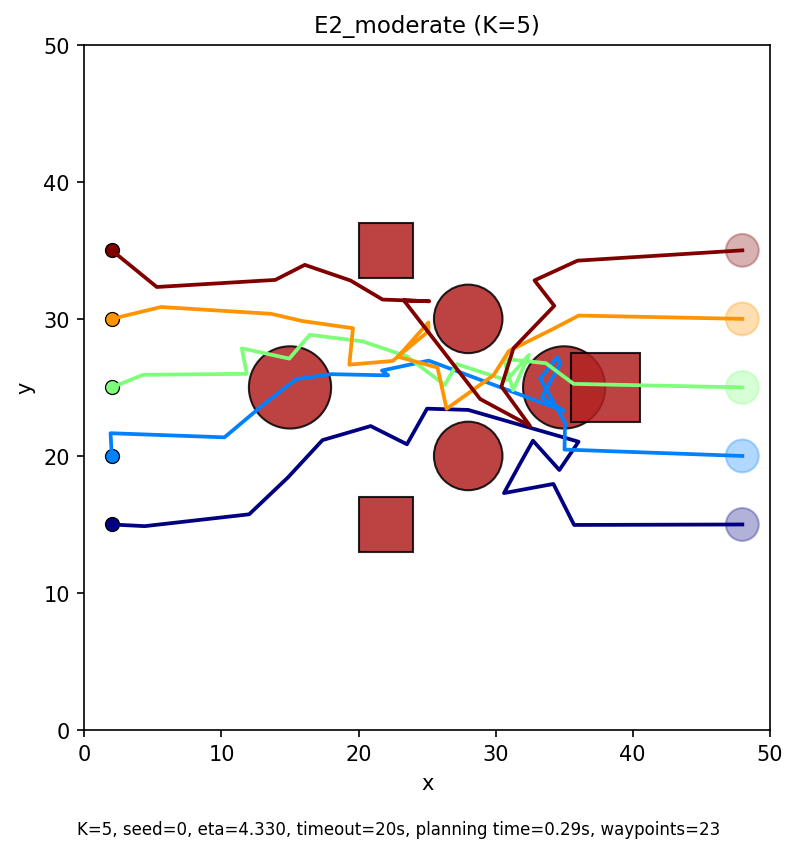
\includegraphics[width=0.24\textwidth]{../A1_code/results/figures/path_E2_moderate.png}
  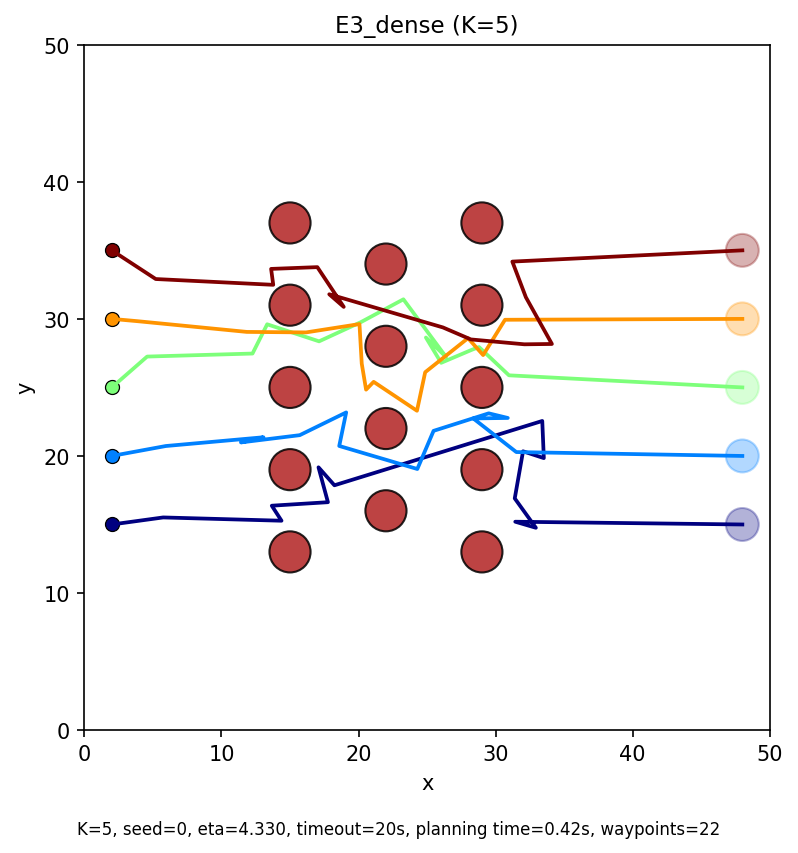
\includegraphics[width=0.24\textwidth]{../A1_code/results/figures/path_E3_dense.png}
  \caption{Successful paths, E0--E3.}
\end{figure}

\begin{figure}[H]
  \centering
  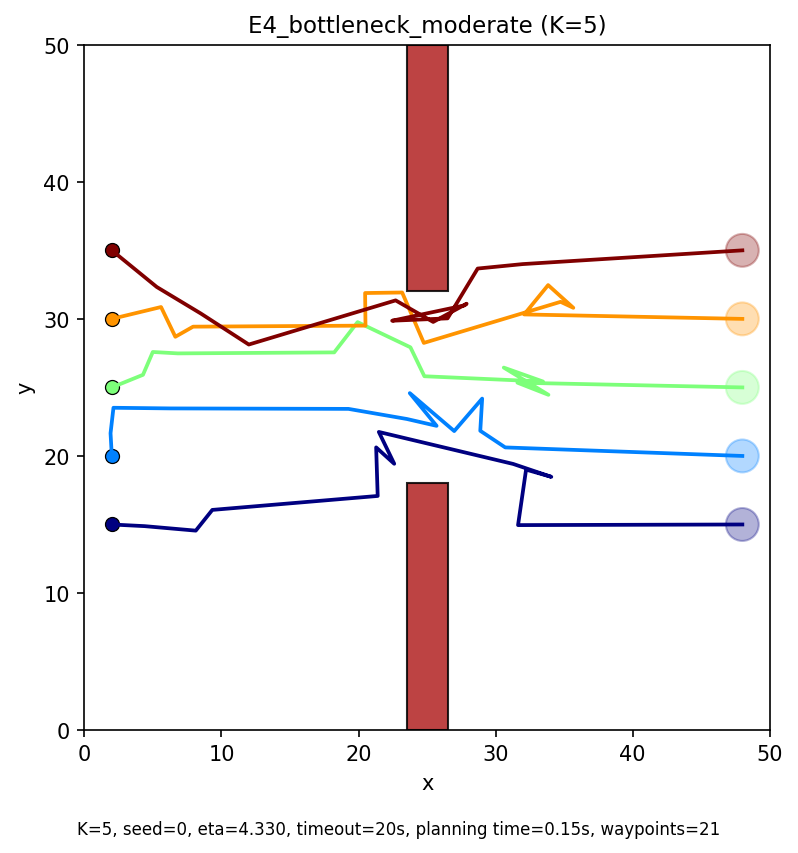
\includegraphics[width=0.24\textwidth]{../A1_code/results/figures/path_E4_bottleneck_moderate.png}
  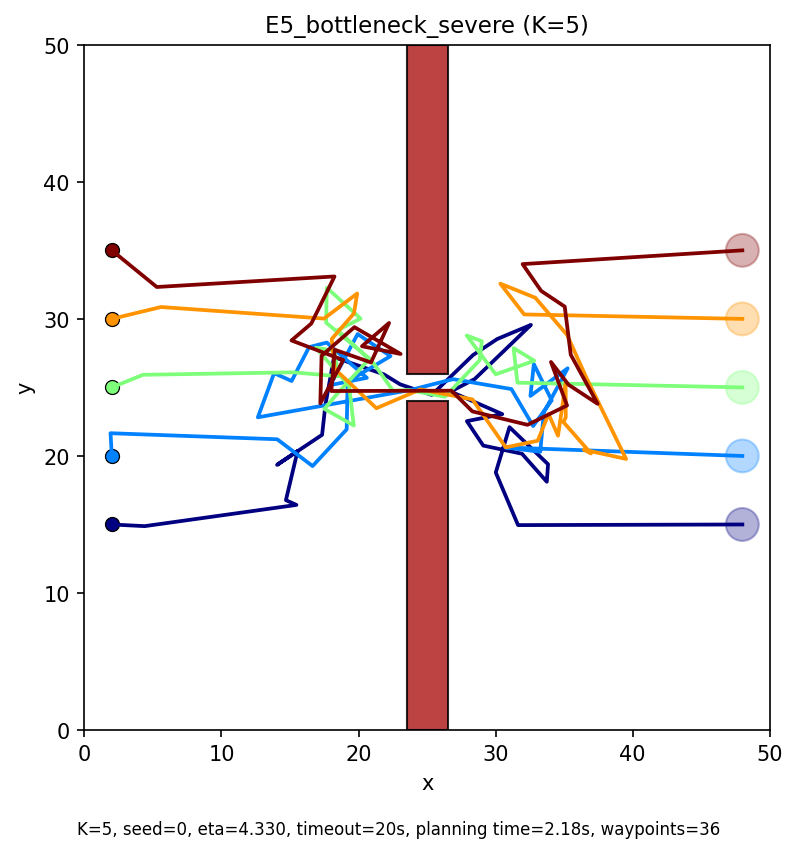
\includegraphics[width=0.24\textwidth]{../A1_code/results/figures/path_E5_bottleneck_severe.png}
  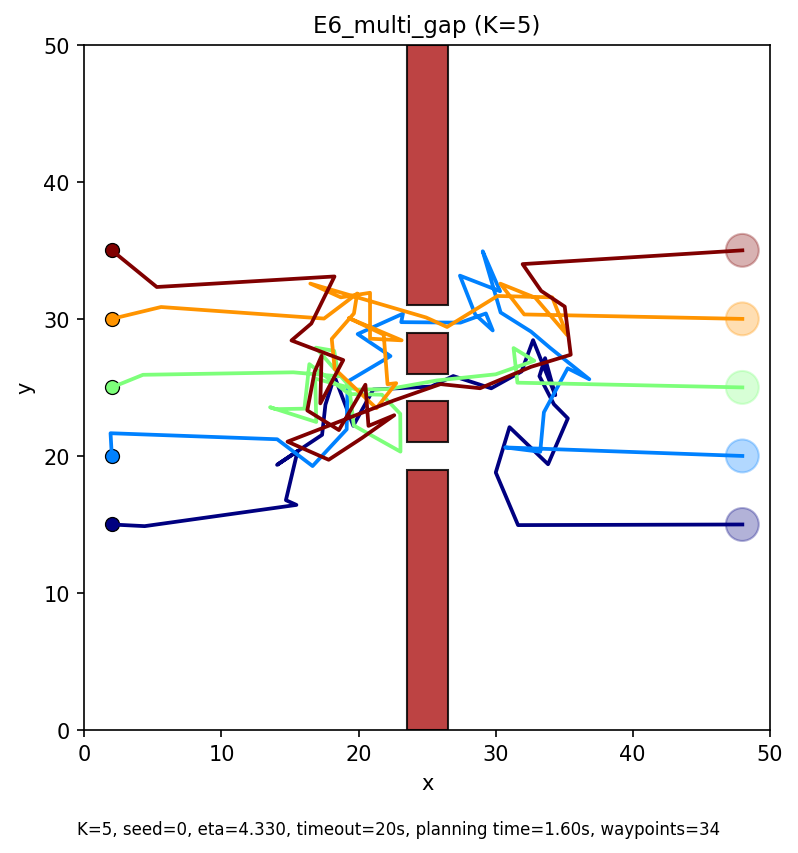
\includegraphics[width=0.24\textwidth]{../A1_code/results/figures/path_E6_multi_gap.png}
  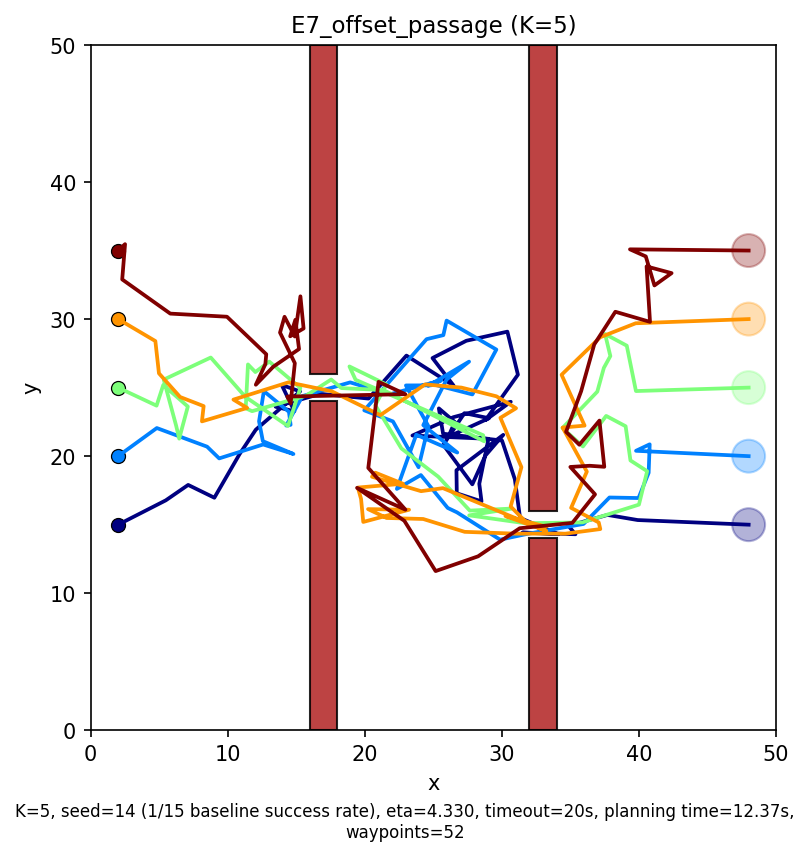
\includegraphics[width=0.24\textwidth]{../A1_code/results/figures/path_E7_offset_passage.png}
  \caption{Successful paths, E4--E7. E7 shows its one success out of 15 seeds.}
\end{figure}

\begin{figure}[H]
  \centering
  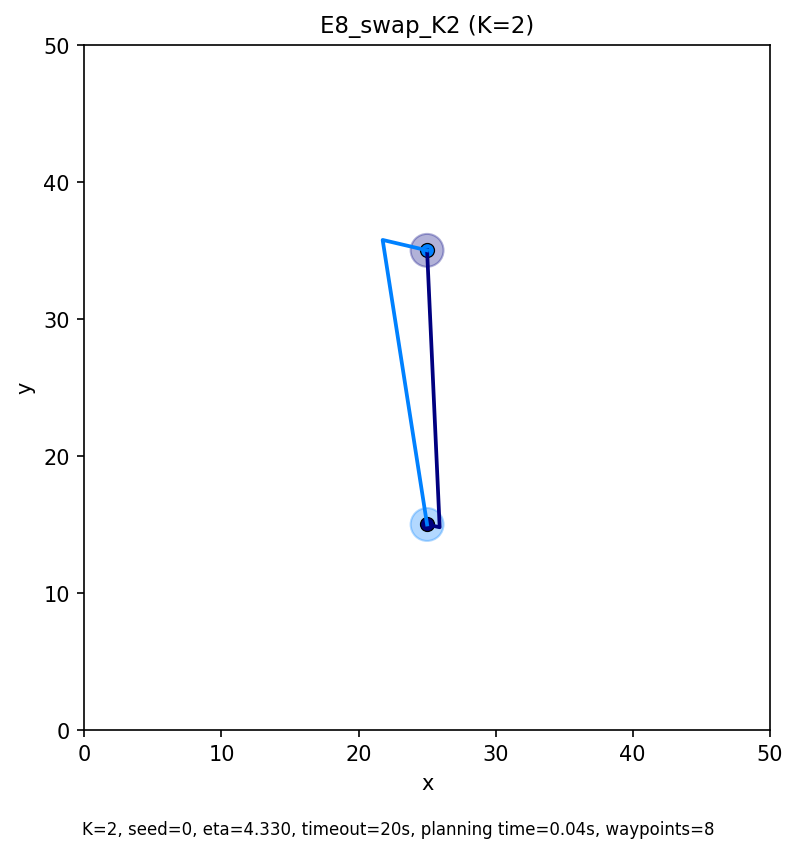
\includegraphics[width=0.24\textwidth]{../A1_code/results/figures/path_E8_swap_K2.png}
  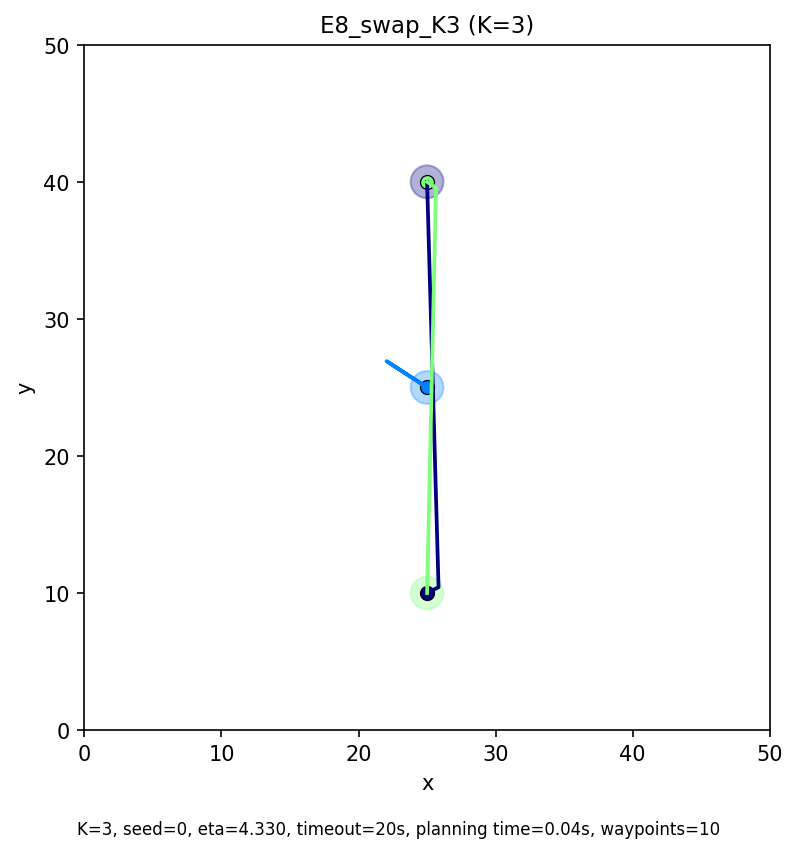
\includegraphics[width=0.24\textwidth]{../A1_code/results/figures/path_E8_swap_K3.png}
  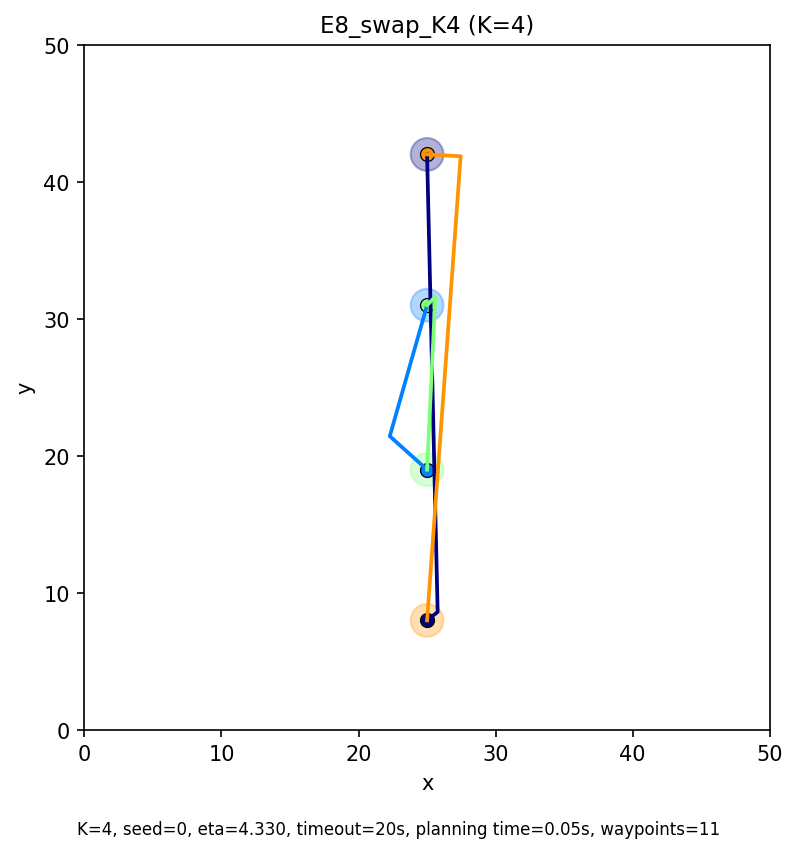
\includegraphics[width=0.24\textwidth]{../A1_code/results/figures/path_E8_swap_K4.png}
  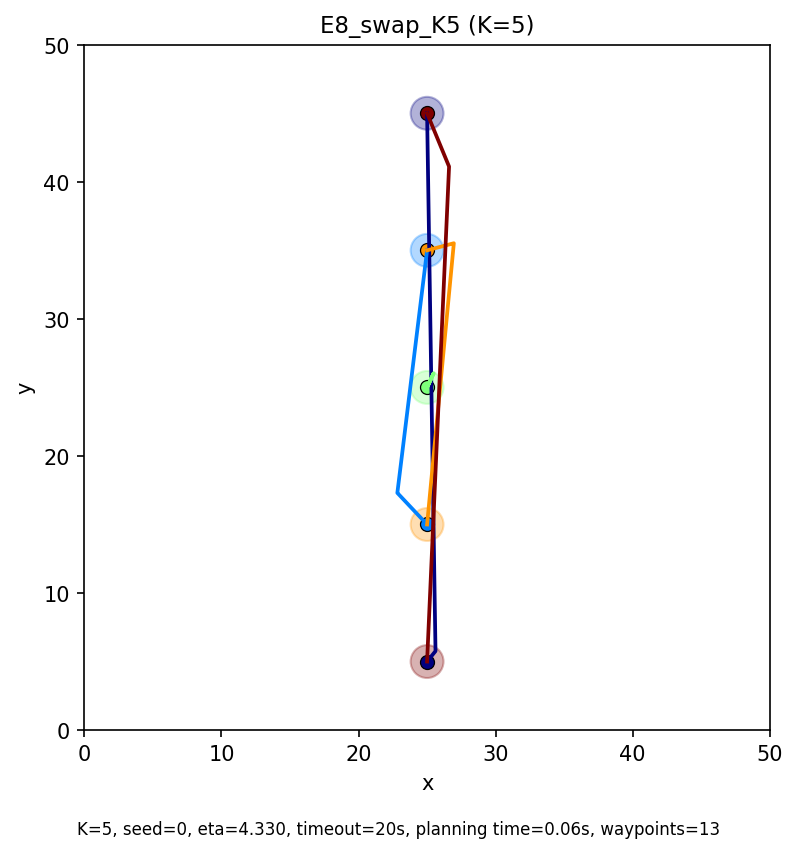
\includegraphics[width=0.24\textwidth]{../A1_code/results/figures/path_E8_swap_K5.png}
  \caption{Successful paths, E8 drone-swap series ($K=2,3,4,5$).}
\end{figure}

\begin{figure}[H]
  \centering
  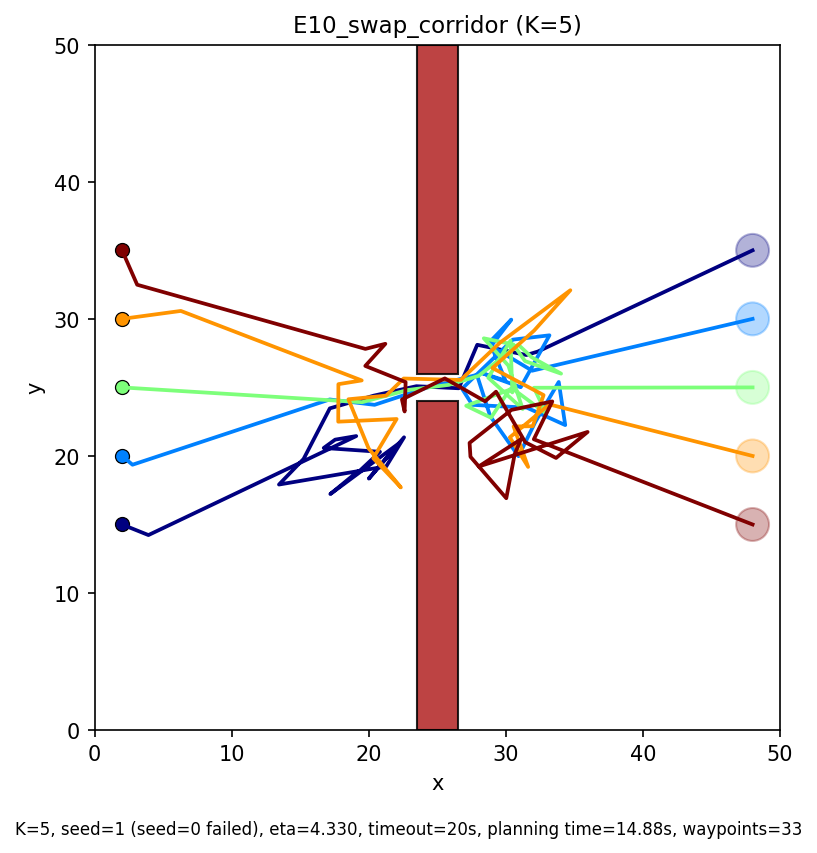
\includegraphics[width=0.24\textwidth]{../A1_code/results/figures/path_E10_swap_corridor.png}
  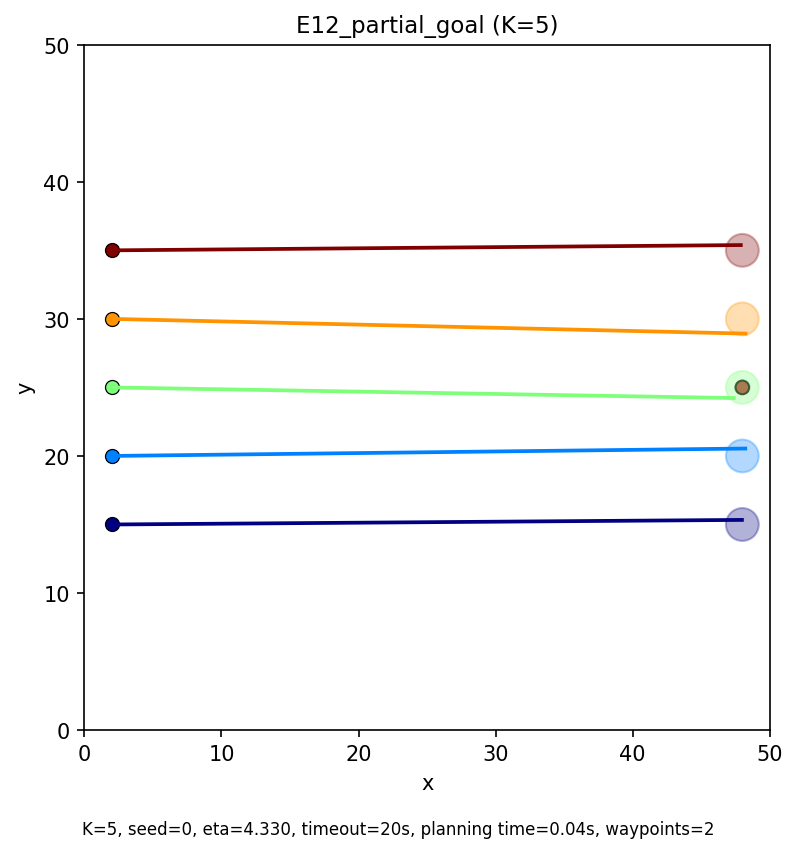
\includegraphics[width=0.24\textwidth]{../A1_code/results/figures/path_E12_partial_goal.png}
  \caption{Successful paths, E10 (bottleneck + drone swap) and E12
  (partial-goal fallback).}
\end{figure}

\end{document}
